\documentclass{standalone}
\usepackage{tikz}
\usepackage{tikz-3dplot}

\usepackage{mathtools}
\usepackage{pgfplots}
\usepackage{graphicx}

\usetikzlibrary{shapes,arrows,matrix,fit,positioning,decorations.pathreplacing,3d,calc}
\usepgfplotslibrary{groupplots}
\usepackage{pgfplotstable}
\usepackage{filecontents}

\pgfplotsset{compat=1.11}
\usepackage{mathpazo} 

\begin{document}

\newcommand{\graphx}{5cm}
\newcommand{\graphy}{4cm}
\newcommand{\piterzi}{60}

\begin{tikzpicture}[>=latex]
	\pgfmathsetlengthmacro{\radius}{sqrt(3)*\graphx}
	\node [circle, minimum width=\radius] (refer) {};
	%\node [circle, draw, minimum width=\radius-1cm] {};
	\draw [|->](0,0.5*\radius-0.5cm) arc(90:360+80:0.5*\radius-0.5cm);
	\node [rotate=60] {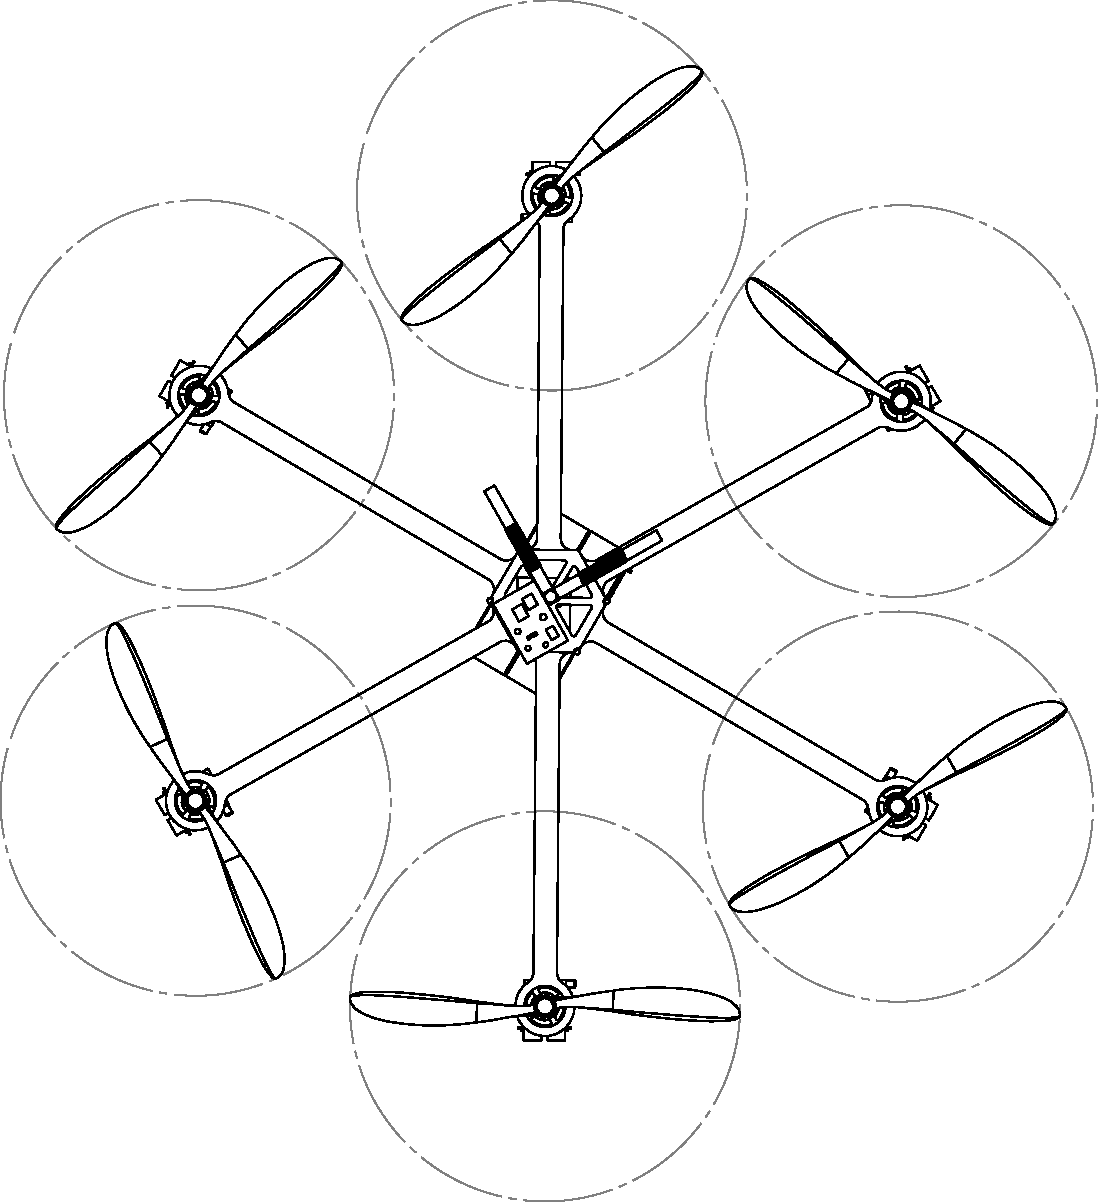
\includegraphics[width=\radius-2cm]{../../img/hexacopterC.pdf}};
	\draw [->](0,0) -- (0,3.5cm) node[anchor=west] {$x$};
	\draw [->](0,0) -- (-3.5cm,0) node[anchor=north] {$y$};
	
	
	\node [rectangle, at=(refer.north), anchor=south, minimum width=\graphx, minimum height=\graphy] (0pi) {};		
	\node [rectangle, at=(0pi.south west), rotate=\piterzi, anchor=south east, minimum width=\graphx, minimum height=\graphy] (pi3) {};		
	\node [rectangle, at=(pi3.south west), rotate=2*\piterzi, anchor=south east, minimum width=\graphx, minimum height=\graphy] (2pi3) {};		
	\node [rectangle, at=(2pi3.south west), rotate=3*\piterzi, anchor=south east, minimum width=\graphx, minimum height=\graphy] (pi) {};		
	\node [rectangle, at=(pi.south west), rotate=4*\piterzi, anchor=south east, minimum width=\graphx, minimum height=\graphy] (4pi3) {};	
	\node [rectangle, at=(4pi3.south west), rotate=5*\piterzi, anchor=south east, minimum width=\graphx, minimum height=\graphy] (5pi3) {};
	
	\begin{axis}[at={(0pi.center)}, anchor=center, rotate=0*\piterzi, width=\graphx, height=\graphy, 
					domain=0:7, ymin=0, ymax=6, xmin=0, xmax=150, 
					grid style={color=gray!40,dotted}, grid=major,
					enlargelimits=false, tick label style={font=\scriptsize},
					xlabel={Time (s)}, ylabel={Distance $d_0$ (m)}]
		\addplot [mark=none, color=black, unbounded coords=jump] table{data/RangeReading4_data.txt};
	\end{axis}	
	\begin{axis}[at={(pi3.center)}, anchor=center, rotate=1*\piterzi, width=\graphx, height=\graphy, 
					domain=0:7, ymin=0, ymax=6, xmin=0, xmax=150, 
					grid style={color=gray!40,dotted}, grid=major,
					enlargelimits=false, tick label style={font=\scriptsize},
					xlabel={Time (s)}, ylabel={Distance $d_{\pi/3}$ (m)},
					x tick label style={anchor=north west}, y tick label style={anchor=north east},
					y label style={rotate=-90-30, anchor=north}, x label style={rotate=60, anchor=north,yshift=-2.5}]
		\addplot [mark=none, color=black, unbounded coords=jump] table{data/RangeReading2_data.txt};
	\end{axis}
	\begin{axis}[at={(2pi3.center)}, anchor=center, rotate=2*\piterzi, width=\graphx, height=\graphy, 
					domain=0:7, ymin=0, ymax=6, xmin=0, xmax=150, 
					grid style={color=gray!40,dotted}, grid=major,
					enlargelimits=false, tick label style={font=\scriptsize},
					xlabel={Time (s)}, ylabel={Distance $d_{2\pi/3}$ (m)},
					x tick label style={anchor=south west}, y tick label style={anchor=north west},
					y label style={rotate=-90+30, anchor=north, yshift=-15}, x label style={rotate=-60, anchor=south, yshift=15}]
		\addplot [mark=none, color=black, unbounded coords=jump] table{data/RangeReading6_data.txt};
	\end{axis}
	\begin{axis}[at={(pi.center)}, anchor=center, rotate=3*\piterzi, width=\graphx, height=\graphy, 
					domain=0:7, ymin=0, ymax=6, xmin=0, xmax=150, 
					grid style={color=gray!40,dotted}, grid=major,
					enlargelimits=false, tick label style={font=\scriptsize},
					xlabel={Time (s)}, ylabel={Distance $d_{\pi}$ (m)},
					x tick label style={anchor=south}, y tick label style={anchor=west},
					y label style={anchor=north, yshift=-10}, x label style={anchor=south, yshift=10}]
		\addplot [mark=none, color=black, unbounded coords=jump] table{data/RangeReading1_data.txt};
	\end{axis}
	\begin{axis}[at={(4pi3.center)}, anchor=center, rotate=4*\piterzi, width=\graphx, height=\graphy, 
					domain=0:7, ymin=0, ymax=6, xmin=0, xmax=150, 
					grid style={color=gray!40,dotted}, grid=major,
					enlargelimits=false, tick label style={font=\scriptsize},
					xlabel={Time (s)}, ylabel={Distance $d_{4\pi/3}$ (m)},
					x tick label style={anchor=south east}, y tick label style={anchor=south west},
					y label style={anchor=south, rotate=-90-30, yshift=10}, x label style={anchor=south, rotate=60,yshift=15}]
		\addplot [mark=none, color=black, unbounded coords=jump] table{data/RangeReading5_data.txt};
	\end{axis}
	\begin{axis}[at={(5pi3.center)}, anchor=center, rotate=5*\piterzi, width=\graphx, height=\graphy, 
					domain=0:7, ymin=0, ymax=6, xmin=0, xmax=150, 
					grid style={color=gray!40,dotted}, grid=major,
					enlargelimits=false, tick label style={font=\scriptsize},
					xlabel={Time (s)}, ylabel={Distance $d_{5\pi/3}$ (m)},
					x tick label style={anchor=north east}, y tick label style={anchor=south east},
					y label style={anchor=south, rotate=-60}, x label style={anchor=south, rotate=-60, yshift=-18.5}]
		\addplot [mark=none, color=black, unbounded coords=jump] table{data/RangeReading3_data.txt};
	\end{axis}

\end{tikzpicture}
\end{document}
